% Created 2023-08-27 Sun 05:39
% Intended LaTeX compiler: pdflatex
\documentclass[11pt]{article}
\usepackage[utf8]{inputenc}
\usepackage[T1]{fontenc}
\usepackage{graphicx}
\usepackage{longtable}
\usepackage{wrapfig}
\usepackage{rotating}
\usepackage[normalem]{ulem}
\usepackage{amsmath}
\usepackage{amssymb}
\usepackage{capt-of}
\usepackage{hyperref}
\usepackage{tikz}
\date{\today}
\title{Bonk-editing}
\hypersetup{
 pdfauthor={},
 pdftitle={Bonk-editing},
 pdfkeywords={},
 pdfsubject={},
 pdfcreator={Emacs 30.0.50 (Org mode 9.7-pre)}, 
 pdflang={English}}
\begin{document}

\maketitle
\tableofcontents

\section{Provide}
\label{sec:orgf69545d}

\begin{verbatim}

(provide 'bonk-editing)

\end{verbatim}
\section{Org Mode}
\label{sec:orgbf554ec}

\subsection{Something hacky to stop org-capture from fucking with my windows order}
\label{sec:orgbd3073f}
\begin{verbatim}
(defun my-org-capture-place-template-dont-delete-windows (oldfun &rest args)
  (cl-letf (((symbol-function 'delete-other-windows) 'ignore))
    (apply oldfun args)))

(with-eval-after-load "org-capture"
  (advice-add 'org-capture-place-template :around 'my-org-capture-place-template-dont-delete-windows))


\end{verbatim}
\subsection{Basic configuration}
\label{sec:org2486a3c}
\begin{verbatim}

(defun bonk/org-no-line-number ()
    (display-line-numbers-mode 0))

(setup (:pkg org :straight t)
    (:hook visual-line-mode visual-fill-column-mode org-init-org-directory-h) 
    (:also-load org-tempo)
    (setq org-ellipsis " ▾"
          org-hide-emphasis-markers t
          org-src-fontify-natively t
          org-fontify-quote-and-verse-blocks t
          org-src-tab-acts-natively t
          org-edit-src-content-indentation 2
          org-hide-block-startup nil
          org-src-preserve-indentation nil
          org-startup-folded 'content
          org-cycle-separator-lines 2
          org-capture-bookmark nil)
    (setq org-refile-targets '((nil :maxlevel . 3)
                               (org-agenda-files :maxlevel . 3)))
    (setq org-outline-path-complete-in-steps nil)

    (setq org-todo-keywords
          '((sequence "TODO(t)" "NEXT(n)" "|" "DONE(d!)")
            (sequence "BACKLOG(b)" "PLAN(p)" "READY(r)" "ACTIVE(a)" "REVIEW(v)" "WAIT(w@/!)" "HOLD(h)" "|" "COMPLETED(c)" "CANC(k@)")))
    (setq org-refile-use-outline-path t)
    (org-babel-do-load-languages
     'org-babel-load-languages
     '((emacs-lisp . t)
       ))


    (push '("conf-unix" . conf-unix) org-src-lang-modes))

\end{verbatim}

\textbf{Guix Packages}

\begin{verbatim}

"emacs-org"

\end{verbatim}
\subsection{Fonts and Bullets}
\label{sec:org9ddf3d0}

Use bullet characters instead of asterisks, plus set the header font sizes to something more palatable.  A fair amount of inspiration has been taken from \href{https://zzamboni.org/post/beautifying-org-mode-in-emacs/}{this blog post}.

\begin{verbatim}

    (setup (:pkg org-superstar :straight t)
      (:load-after org)
      (:hook-into org-mode)
      (:option org-superstar-remove-leading-stars t
               org-superstar-headline-bullets-list '("◉" "○" "●" "○" "●" "○" "●")))

;; Replace list hyphen with dot
;; (font-lock-add-keywords 'org-mode
;;                         '(("^ *\\([-]\\) "
;;                             (0 (prog1 () (compose-region (match-beginning 1) (match-end 1) "•"))))))

(setup org-faces
    ;; Make sure org-indent face is available
    (:also-load org-indent)
    (:when-loaded
      ;; Increase the size of various headings
      (set-face-attribute 'org-document-title nil :font "Hack Nerd Font" :weight 'bold :height 1.3)

      (dolist (face '((org-level-1 . 1.2)
                      (org-level-2 . 1.1)
                      (org-level-3 . 1.05)
                      (org-level-4 . 1.0)
                      (org-level-5 . 1.1)
                      (org-level-6 . 1.1)
                      (org-level-7 . 1.1)
                      (org-level-8 . 1.1)))
        (set-face-attribute (car face) nil :font "Hack Nerd Font" :weight 'medium :height (cdr face)))

      ;; Ensure that anything that should be fixed-pitch in Org files appears that way
      (set-face-attribute 'org-block nil :foreground nil :inherit 'fixed-pitch)
      (set-face-attribute 'org-table nil  :inherit 'fixed-pitch)
      (set-face-attribute 'org-formula nil  :inherit 'fixed-pitch)
      (set-face-attribute 'org-code nil   :inherit '(shadow fixed-pitch))
      (set-face-attribute 'org-indent nil :inherit '(org-hide fixed-pitch))
      (set-face-attribute 'org-verbatim nil :inherit '(shadow fixed-pitch))
      (set-face-attribute 'org-special-keyword nil :inherit '(font-lock-comment-face fixed-pitch))
      (set-face-attribute 'org-meta-line nil :inherit '(font-lock-comment-face fixed-pitch))
      (set-face-attribute 'org-checkbox nil :inherit 'fixed-pitch)

      ;; Get rid of the background on column views
      (set-face-attribute 'org-column nil :background nil)
      (set-face-attribute 'org-column-title nil :background nil)))

;; TODO: Others to consider
;; '(org-document-info-keyword ((t (:inherit (shadow fixed-pitch)))))
;; '(org-meta-line ((t (:inherit (font-lock-comment-face fixed-pitch)))))
;; '(org-property-value ((t (:inherit fixed-pitch))) t)
;; '(org-special-keyword ((t (:inherit (font-lock-comment-face fixed-pitch)))))
;; '(org-table ((t (:inherit fixed-pitch :foreground "#83a598"))))
;; '(org-tag ((t (:inherit (shadow fixed-pitch) :weight bold :height 0.8))))
;; '(org-verbatim ((t (:inherit (shadow fixed-pitch))))))

\end{verbatim}

\textbf{Guix Packages}

\begin{verbatim}

"emacs-org-superstar"

\end{verbatim}
\subsection{Block Templates}
\label{sec:orgc857590}

These templates enable you to type things like \texttt{<el} and then hit \texttt{Tab} to expand
the template.  More documentation can be found at the Org Mode \href{https://orgmode.org/manual/Easy-templates.html}{Easy Templates}
documentation page.

\begin{verbatim}
;; This is needed as of Org 9.2
(setup org-tempo
    (:when-loaded
      (add-to-list 'org-structure-template-alist '("sh" . "src sh"))
      (add-to-list 'org-structure-template-alist '("py" . "src python"))
      (add-to-list 'org-structure-template-alist '("el" . "src emacs-lisp"))
      (add-to-list 'org-structure-template-alist '("scm" . "src scheme"))
      (add-to-list 'org-structure-template-alist '("li" . "src lisp"))
      (add-to-list 'org-structure-template-alist '("rb" . "src ruby"))
      (add-to-list 'org-structure-template-alist '("js" . "src javascript"))
      (add-to-list 'org-structure-template-alist '("cpp" . "src C++"))
      (add-to-list 'org-structure-template-alist '("ts" . "src typescript"))
      (add-to-list 'org-structure-template-alist '("py" . "src python"))
      (add-to-list 'org-structure-template-alist '("go" . "src go"))
      (add-to-list 'org-structure-template-alist '("yaml" . "src yaml"))
      (add-to-list 'org-structure-template-alist '("r" . "src R :noweb yes :exports both"))
      (add-to-list 'org-structure-template-alist '("json" . "src json"))))


\end{verbatim}
\subsection{Org file type insertion}
\label{sec:orge653f19}
I know i could use org-capture-templates for this, but i don't want to apply
this automatically or in a predefined way. Perhaps there is a more elegant or
comfy way of doing this but well\ldots{}

\begin{verbatim}

(defun prob-buffer (buffer-name)
    "Creates a new probability and statistics buffer for school."
    (interactive "sSet new buffer Name: ")
    (let (($buf (generate-new-buffer buffer-name)))
      (switch-to-buffer $buf)
      (insert
       "#+author:\n#+TITLE:
#+LATEX_HEADER: \\usepackage{unicode-math}
#+LATEX_HEADER: \\usepackage{amsfonts}
#+STARTUP: latexpreview
#+OPTIONS: toc:t
#+LATEX_CLASS: article
#+LATEX_CLASS_OPTIONS: [a5paper, landscape]
#+BABEL: noweb yes
#+PROPERTY: header-args:python :session practica1 :results output
#+PROPERTY: header-args:python+ :async yes :results output")
      (funcall 'org-mode)
      (setq buffer-offer-save t)))


\end{verbatim}
\subsection{Agenda}
\label{sec:org8e8a6d0}
\begin{verbatim}
      (defun org-init-org-directory-h ()
        (setq org-directory "~/Notes/agenda/")
        (unless org-id-locations-file
          (setq org-id-locations-file (expand-file-name ".orgids" org-directory))))

    (defun org-init-agenda-h ()
      (setq org-agenda-files (list org-directory)))
      (setq
       ;; Different colors for different priority levels
       org-agenda-deadline-faces
       '((1.001 . error)
         (1.0 . org-warning)
         (0.5 . org-upcoming-deadline)
         (0.0 . org-upcoming-distant-deadline))
       ;; Don't monopolize the whole frame just for the agenda
       org-agenda-window-setup 'current-window
       org-agenda-skip-unavailable-files t
       ;; Shift the agenda to show the previous 3 days and the next 7 days for
       ;; better context on your week. The past is less important than the future.
       org-agenda-span 10
       org-agenda-start-on-weekday nil
       org-agenda-start-day "-3d"
       ;; Optimize `org-agenda' by inhibiting extra work while opening agenda
       ;; buffers in the background. They'll be "restarted" if the user switches to
       ;; them anyway (see `+org-exclude-agenda-buffers-from-workspace-h')
       org-agenda-inhibit-startup t)
    (setup (:pkg org-agenda)
      (:hook org-init-agenda-h)

      (setq org-agenda-custom-commands
            '(("d" "Dashboard"
               ((agenda "" ((org-deadline-warning-days 7)))
                (todo "NEXT"
                      ((org-agenda-overriding-header "Next Tasks")))
                (tags-todo "agenda/ACTIVE" ((org-agenda-overriding-header "Active Projects")))))

      ("n" "Next Tasks"
       ((todo "NEXT"
          ((org-agenda-overriding-header "Next Tasks")))))


      ("W" "Work Tasks" tags-todo "+work")

      ;; Low-effort next actions
      ("e" tags-todo "+TODO=\"NEXT\"+Effort<15&+Effort>0"
       ((org-agenda-overriding-header "Low Effort Tasks")
        (org-agenda-max-todos 20)
        (org-agenda-files org-agenda-files)))

      ("w" "Workflow Status"
       ((todo "WAIT"
              ((org-agenda-overriding-header "Waiting on External")
               (org-agenda-files org-agenda-files)))
        (todo "REVIEW"
              ((org-agenda-overriding-header "In Review")
               (org-agenda-files org-agenda-files)))
        (todo "PLAN"
              ((org-agenda-overriding-header "In Planning")
               (org-agenda-todo-list-sublevels nil)
               (org-agenda-files org-agenda-files)))
        (todo "BACKLOG"
              ((org-agenda-overriding-header "Project Backlog")
               (org-agenda-todo-list-sublevels nil)
               (org-agenda-files org-agenda-files)))
        (todo "READY"
              ((org-agenda-overriding-header "Ready for Work")
               (org-agenda-files org-agenda-files)))
        (todo "ACTIVE"
              ((org-agenda-overriding-header "Active Projects")
               (org-agenda-files org-agenda-files)))
        (todo "COMPLETED"
              ((org-agenda-overriding-header "Completed Projects")
               (org-agenda-files org-agenda-files)))
        (todo "CANC"
              ((org-agenda-overriding-header "Cancelled Projects")
               (org-agenda-files org-agenda-files)))))))
      )

(define-key global-map (kbd "C-c j")
    (lambda () (interactive) (org-capture nil "j")))
\end{verbatim}
\subsection{Capture Templates}
\label{sec:org728d7a8}
\begin{verbatim}

(setq org-capture-templates
  `(("t" "Tasks / Projects")
    ("tt" "Task" entry (file "Tasks.org")
         "* TODO %?\n  %U\n  %a\n  %i" :empty-lines 1)
      ("o" "Centralized templates for projects")
      ("ot" "Project todo" entry
       (file "Projects_todo.org")
       "* TODO %?\n %i\n %a"
       :heading "Tasks"
       :prepend nil)
      ("on" "Project notes" entry
       (file+headline "Projects_notes.org" "Project Notes")
       "* %U %?\n %i\n %a"
       :heading "Notes"
       :prepend t)
      ("oc" "Project changelog" entry
       (file "Project_Changelog.org")
       "* %U %?\n %i\n %a"
       :heading "Changelog"
       :prepend t)

    ("j" "Journal Entries")
    ("jj" "Journal" entry
         (file+olp+datetree "Journal.org")
         "\n* %<%I:%M %p> - Journal :journal:\n\n%?\n\n"
         ;; ,(dw/read-file-as-string "~/Notes/Templates/Daily.org")
         :clock-in :clock-resume
         :empty-lines 1)
    ("jm" "Meeting" entry
         (file+olp+datetree "Journal.org")
         "* %<%I:%M %p> - %a :meetings:\n\n%?\n\n"
         :clock-in :clock-resume
         :empty-lines 1)

    ("w" "Workflows")
    ("we" "Checking Email" entry (file+olp+datetree "Wokr.org")
         "* Checking Email :email:\n\n%?" :clock-in :clock-resume :empty-lines 1)

    ("m" "Metrics Capture")
    ("mw" "Weight" table-line (file+headline "Metrics.org" "Weight")
     "| %U | %^{Weight} | %^{Notes} |" :kill-buffer t)))
\end{verbatim}
\subsection{Pomodoro}
\label{sec:orgd947148}

\begin{verbatim}

(setup (:pkg org-pomodoro :straight t)

  (bonk/set-leader-keys
    "op"  '(org-pomodoro :which-key "pomodoro")))

\end{verbatim}

\textbf{Guix Packages}

\begin{verbatim}

"emacs-org-pomodoro"

\end{verbatim}
\subsection{Protocol}
\label{sec:org4816c36}

This is probably not needed if I plan to use custom functions that are invoked
through \texttt{emacsclient.}

\begin{verbatim}

(require 'org-protocol)

\end{verbatim}
\subsection{Center Org Buffers}
\label{sec:orgdfc6688}
\begin{verbatim}

(defun bonk/org-mode-visual-fill ()
      (setq visual-fill-column-center-text t)
      (setq visual-fill-column-width 100)
      (visual-fill-column-mode 1))

(setup (:pkg visual-fill-column :straight t)
    (:hook-into org)
    (bonk/org-mode-visual-fill))

\end{verbatim}
\subsection{Bindings}
\label{sec:org0382bc7}

\begin{verbatim}

(setup (:pkg evil-org :straight t)
    (:hook-into org-mode org-agenda-mode)
    (require 'evil-org)
    (require 'evil-org-agenda)
    (evil-org-set-key-theme '(navigation todo insert textobjects additional))
    (evil-org-agenda-set-keys))

(bonk/set-leader-keys
    "o"   '(:ignore t :which-key "org mode")

    "oi"  '(:ignore t :which-key "insert")
    "oil" '(org-insert-link :which-key "insert link")

    "on"  '(org-toggle-narrow-to-subtree :which-key "toggle narrow")

    "olp" '(org-latex-preview :which-key "preview latex block")

    "oa"  '(org-agenda :which-key "status")
    "ot"  '(org-todo-list :which-key "todos")
    "oc"  '(org-capture t :which-key "capture")
    "ox"  '(org-export-dispatch t :which-key "export"))

\end{verbatim}

\textbf{Guix Packages}

\begin{verbatim}

"emacs-evil-org"

\end{verbatim}
\subsection{Configure Babel Languages}
\label{sec:org15ced7e}

To execute or export code in \texttt{org-mode} code blocks, you'll need to set up \texttt{org-babel-load-languages} for each language you'd like to use.  \href{https://orgmode.org/worg/org-contrib/babel/languages.html}{This page} documents all of the languages that you can use with \texttt{org-babel}.

\begin{verbatim}
      (setup (:pkg ob-rust :straight t))
      (setup (:pkg ob-go :straight t))
      (setup (:pkg ob-typescript :straight t))
      (setup (:pkg ob-ipython :straight t))
(setup (:pkg ob-sagemath :straight t))
(setup (:pkg jupyter :straight t))
      (with-eval-after-load 'org
        (org-babel-do-load-languages
          'org-babel-load-languages
          '((emacs-lisp . t)
            (python . t)
            (R . t)
            (typescript . t)
            (go . t)
            (scheme . t)
            (rust . t)
            (lisp . t)))
        (setq org-confirm-babel-evaluate nil)
        (setq org-babel-lisp-eval-fn #'sly-eval)

        (push '("conf-unix" . conf-unix) org-src-lang-modes))
\end{verbatim}
\subsection{Org Present}
\label{sec:orgc80f022}
\texttt{org-present}
\begin{verbatim}
(defun bonk/org-present-prepare-slide ()
  (org-overview)
  (org-show-entry)
  (org-show-children))

(defun bonk/org-present-hook ()
  (setq header-line-format " ")
  (org-appear-mode -1)
  (org-display-inline-images)
  (bonk/org-present-prepare-slide))

(defun bonk/org-present-quit-hook ()
  (setq header-line-format nil)
  (org-present-small)
  (org-remove-inline-images)
  (org-appear-mode 1))

(defun bonk/org-present-prev ()
  (interactive)
  (org-present-prev)
  (bonk/org-present-prepare-slide))

(defun bonk/org-present-next ()
  (interactive)
  (org-present-next)
  (bonk/org-present-prepare-slide)
  (when (fboundp 'live-crafter-add-timestamp)
    (live-crafter-add-timestamp (substring-no-properties (org-get-heading t t t t)))))

(setup (:pkg org-present)
  (:with-map org-present-mode-keymap
    (:bind "C-c C-j" bonk/org-present-next
           "C-c C-k" bonk/org-present-prev))
  (:hook bonk/org-present-hook)
  (:with-hook org-present-mode-quit-hook
    (:hook bonk/org-present-quit-hook)))
\end{verbatim}
\subsection{Org-tikz (graphs and stuff preview)}
\label{sec:org656cf2f}
\begin{verbatim}
(setup (:pkg texfrag :straight t))
(add-hook 'org-mode-hook
  (lambda ()
    (texfrag-mode)
  ))

(add-to-list 'org-latex-packages-alist
             '("" "tikz" t))
(eval-after-load "preview"
  '(add-to-list 'preview-default-preamble "\\PreviewEnvironment{tikzpicture}" t))
\end{verbatim}
\subsubsection{Keymaps}
\label{sec:orgce15be1}

\begin{center}
\begin{tabular}{ll}
Value & function\\[0pt]
-------- & ------------------------------\\[0pt]
<left> & org-present-prev\\[0pt]
<right> & org-present-next\\[0pt]
C-c   < & org-present-beginning\\[0pt]
C-c   > & org-present-end\\[0pt]
C-c   C-- & org-present-small\\[0pt]
C-c   C-1 & org-present-toggle-one-big-page\\[0pt]
C-c   C-= & org-present-big\\[0pt]
C-c   C-q & org-present-quit\\[0pt]
C-c   C-r & org-present-read-only\\[0pt]
C-c   C-w & org-present-read-write\\[0pt]
\end{tabular}
\end{center}
\subsection{{\bfseries\sffamily TODO} Update Table of Contents on Save}
\label{sec:org5f526d4}

It's nice to have a table of contents section for long literate configuration files (like this one!) so I use \texttt{org-make-toc} to automatically update the ToC in any header with a property named \texttt{TOC}.

\begin{verbatim}

(setup (:pkg org-make-toc :straight t)
  (:hook-into org-mode))

\end{verbatim}

\textbf{Guix Packages}

\begin{verbatim}

"emacs-org-make-toc"

\end{verbatim}
\section{Buffer-alist}
\label{sec:org9b9058f}
\begin{verbatim}

(setopt
 display-buffer-base-action
 '((display-buffer-reuse-window display-buffer-same-window
    display-buffer-in-previous-window
    display-buffer-use-some-window)))
(setopt
 display-buffer-alist
 (cons '("*Org*" (display-buffer-same-window))
        display-buffer-alist))

  (add-to-list 'display-buffer-alist
               '("\\*org-roam\\*"
                    (inhibit-switch-frame . t)
(
                 (window-width . 0.33)
                 (window-parameters . ((no-other-window . t)
                                       (no-delete-other-windows . t))))))
\end{verbatim}
\section{Org-Roam}
\label{sec:orgd7336d6}

\begin{verbatim}
(setup (:pkg org-roam :straight t)
  (setq org-roam-v2-ack t)
  (:when-loaded
    (org-roam-db-autosync-mode))
  (:option
   org-roam-directory "~/Notes/Roam/"
   org-roam-completion-everywhere t
   org-roam-capture-templates
   '(("d" "default" plain "%?"
      :if-new (file+head "%<%Y%m%d%H%M%S>-${slug}.org"
                         "#+title: ${title}\n")
      :unnarrowed t)
     ("l" "learn org roam" plain
      "* Category\n- Class: [[roam:roam]] \n- Topic: %?"
      :if-new (file+head "learn_org_roam/${title}.org"
                         "#+title: ${title}\n#+filetags: org roam learning")
      :unnarrowed t)
     ("p" "programming note" plain
      "* Category\n- Class: [[programming]] \n- Topic: %?\n- Language: "
      :if-new (file+head "programming/${title}.org"
                         "#+title: ${title}\n#+filetags: org roam programming")
      :unnarrowed t)
     ("pg" "programming note with graphics" plain
      "* Category\n- Class: [[programming]] \n- Topic: %?\n- Language: \n #+LATEX_HEADER: \\usepackage{tikz}\n#+LATEX_HEADER: \\usepackage{svg}\n#+HEADER: :imagemagick yes\n#+HEADER: :exports results\n#+HEADER: :results output graphics file"
      :if-new (file+head "programming/${title}.org"
                         "#+title: ${title}\n#+filetags: org roam programming graphics")
      :unnarrowed t)
     ("m" "math_esp" plain
      "* Category\n- Class: [[roam:math]] \n- Topic: %?"
      :if-new (file+head "math_esp/${title}.org"
                         "#+title: ${title}\n#+filetags: math esp")
      :unnarrowed t)
     ("D" "math_esp definition" plain
      "* Category\n- Class: [[roam:math]] \n- Topic: %? \n* Definicion"
      :if-new (file+head "math_esp/definitions/${title}.org"
                         "#+title: ${title}\n#+filetags: math esp definitions")
      :unnarrowed t)
     ("E" "math_esp example" plain
      "* Category\n- Class: [[roam:math]] \n- Topic: %? \n* Ejemplos"
      :if-new (file+head "math_esp/examples/${title}.org"
                         "#+title: ${title}\n#+filetags: math esp examples")
      :unnarrowed t)
     ("P" "math_esp properties" plain
      "* Category\n- Class: [[roam:math]] \n- Topic: %? \n* Propiedades"
      :if-new (file+head "math_esp/properties/${title}.org"
                         "#+title: ${title}\n#+filetags: math esp propiedades")
      :unnarrowed t)))
  (:global "C-c n l"   org-roam-buffer-toggle
           "C-c n f"   org-roam-node-find
           "C-c n c"   org-roam-dailies-capture-today
           "C-c n g"   org-roam-graph
           "C-c n i"  org-roam-node-insert))
(setup (:pkg org-roam-ui :straight t))

\end{verbatim}


\begin{verbatim}
((el . src emacs-lisp) (py . src python) (sh . src shell) (a . export ascii) (c . center) (C . comment) (e . example) (E . export) (h . export html) (l . export latex) (q . quote) (s . src) (v . verse))
\end{verbatim}





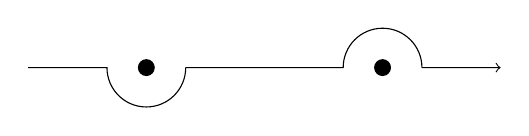
\begin{tikzpicture}
\draw[->] (-3,0) -- (-2,0) arc[radius=0.5cm,start angle=-180,end angle=0] (-1,0) -- (1,0) arc[radius=0.5cm,start angle=180,end angle=0] (2,0) -- (3,0);
\filldraw (-1.5,0) circle[radius=1mm];
\filldraw (1.5,0) circle[radius=1mm];
\end{tikzpicture}
\end{document}